\chapter{Post-transition metal doping of monolayer $WS_2$}

\section{Introduction}

Single layer TMDC materials present a range of unique optical, electrical and mechanical properties which make them promising materials beyond graphene in future nanotechnologies.
Atomic doping can further extend the potential of TMDCs since it has been predicted that a number of properties can be tuned trough compositional variation. Up until now doping has relied on charge transfer induced by changing the environmental conditions such as surface adsorption, metal contacts and dielectric interfaces. This approach has demonstrated to severely limit the device working conditions thus doping trough stable incorporation of non-volatile metal atoms is highly preferred.

Achieving controlled doping is a challenge which is aggravated by the fact that established synthesis protocols for these materials are still lacking.

Doping of monolayer $WS_2$ with post-transition metals has not been reported as yet. Doping of $WS_2$ with post-transition metals can lead to chemisorbed intercalated atoms between layers which can be regarded as analogous to deep level impurities. It can lead to an additional energy level near to the top of the valence band or, alternatively, as a modification of the energy band of the host crystal due to the interaction between the intercalate and W or S atoms \cite{Yacobi1979}\cite{Yacobi1979a}. In particular indium may generate an additional energy state at the top of the valence band which leads to a subsequent upward shift of this band \cite{Deshpande2001}. A gradual increase in this shift with increasing number of intercalating atoms would lead to a linear decrease in the energy gap with increasing In content as observed in In-intercalated bulk $WS_2$ \cite{Deshpande2001}. This led to the demonstration of higher conductivity and photocurrent than both pure $WS_2$ films thus proving to be highly photo-active. Unlike their alkali and alkaline earth metal analogues, In-intercalated bulk WS2 compounds were found to be stable against oxidation when exposed to air or chemical due to a fairly strong guest-host bonding which hinders deintercalation processes and preserving a perfect 2H crystalline phase \cite{Deshpande2001}\cite{Rao1981}. Further, In has lower melting and boiling points than B, Al and Ga enabling doping via CVD or MOCVD synthesis of $WS_2$ at low temperatures. These characteristics make Indium a very interesting prospected dopant of $WS_2$ to pave the way towards applications as photoelectrodes in solar cells. Post transition metals are prone to intercalate between the layers however displaying very different effect with respect to the alkali and alkaline earth metal intercalates of $WS_2$.

Here we demonstrate indium doping of monolayer $WS_2$ in–situ during CVD synthesis of $WS_2$. The process relies on the addition of a volatile indium precursor which results in large-area In-doped $WS_2$ atomic layers exhibiting tunable optical properties and a semiconducting-to-metallic transition at high doping levels. We also demonstrate controlled indium content from 0 up to 45\% in $WS_2$ maintaining a 2D morphology and atomically thin nature of the material without sacrificing the lateral extension and scalability of the synthesis process.

\section{Results}

The CVD synthesis of In-doped $WS_2$ samples was performed by using the optimized conditions to obtain high-optical quality and high-mobility monolayer $WS_2$ \cite{Reale2017}. Here, In(OH)3 powders were added as indium precursor to the W precursor powder and loaded in the center of a quartz tubular furnace (Figure \ref{fig:InFurnaceSetup}). A first indication of the effect of indium in the $WS_2$ is provided by the morphology of the triangular domains. SEM and OM images of $WS_2$ domains grown by using different $In(OH)_3/H_2WO_4$ weight ratios [$In_{0.25}WS_2$, $In_{0.5}WS_2$, $In_{0.75}WS_2$, $In_1WS_2$ (Table \ref{tab:InRatios})] are shown in Figure \ref{fig:InOMSEMImages}. While from the optical contrast it is possible to see that the monolayer nature of the domains is unchanged, it can be noticed how the shape of triangles progressively change. Triangles with straight edges similar to that of pristine $WS_2$ are displayed for low In content while convex and jagged edges appear by increasing the Indium, which might suggest a more significant incorporation of the latter. $WS_2$ with high indium content can also present different morphologies and even large coverage.

\begin{figure}[!h]
	\begin{center}
		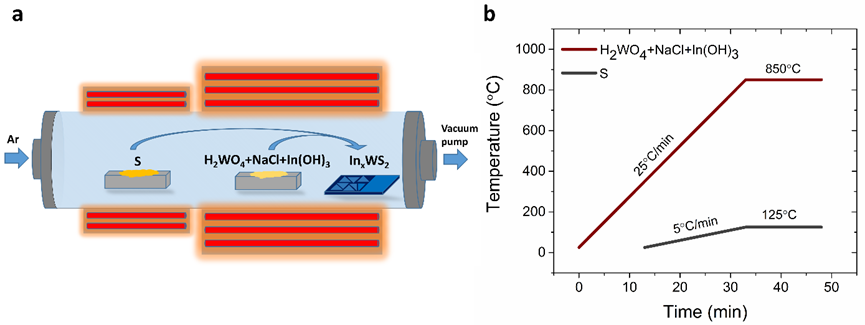
\includegraphics[scale=0.5]{In/FurnaceSetup.png}
		\caption{Illustration of the (a) two-zone CVD tubular furnace set-up and (b) temperature profiles of the W and In precursors-furnace and S-heating module. The S reaches 125 {\degree}C when the main furnace is at 850 {\degree}C. The $SiO_2/Si$ substrate is loaded downstream at 1-8 cm away from the W and In precursors-containing crucible and it is subjected to the same temperature.}
		\label{fig:InFurnaceSetup}
	\end{center}
\end{figure}

The presence of indium has been confirmed by XRD, Raman, PL and XPS characterisations discussed in the following.

\begin{figure}[!ht]
	\begin{center}
		\begin{subfigure}[b]{0.7\textwidth}
			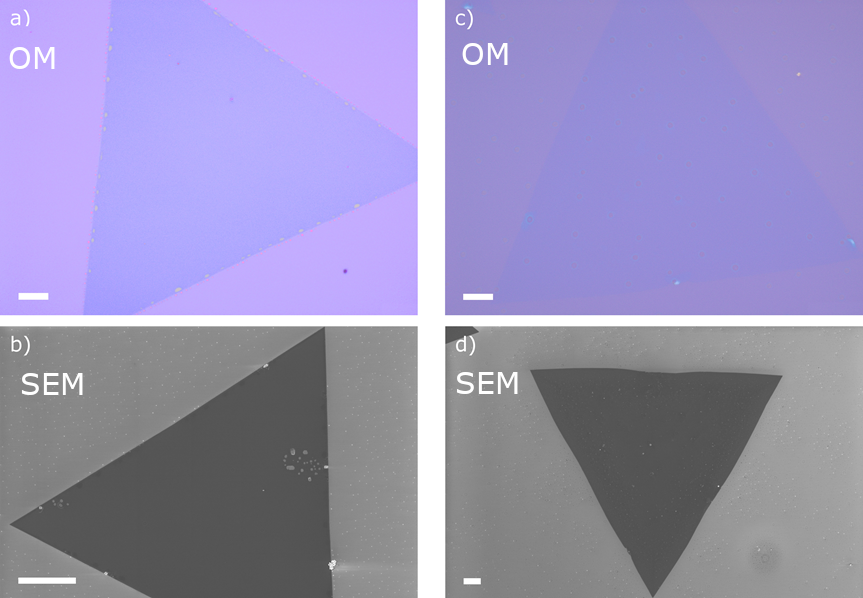
\includegraphics[width=\textwidth]{In/OMSEMImages1.png}
			\label{fig:InOMSEMImages1}
		\end{subfigure}
		\qquad
		\begin{subfigure}[b]{0.7\textwidth}
			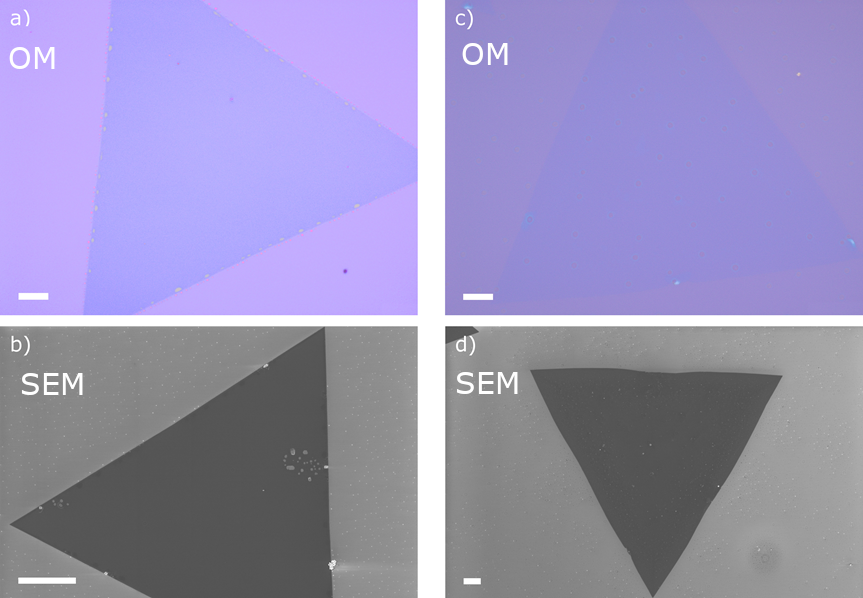
\includegraphics[width=\textwidth]{In/OMSEMImages1.png}
			\label{fig:InOMSEMImages2}
		\end{subfigure}
		\caption{Optical and SEM images of flakes grown by using different $In(OH)_3/H_2WO_4$ weight ratios: (a, b) 0.25, (c, d) 0.5, (e, f) 0.75 and (g, h)=1. All other synthesis conditions and parameters were kept constant as described above (Table S1).}
		\label{fig:InOMSEMImages}
	\end{center}
\end{figure}

\begin{figure}[!h]
	\begin{center}
		\begin{subfigure}[b]{0.6\textwidth}
			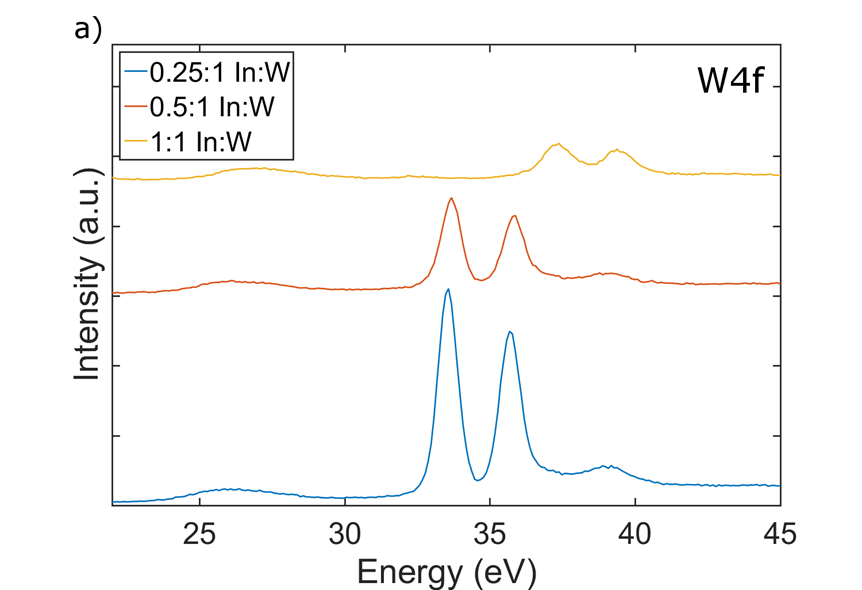
\includegraphics[width=\textwidth]{In/XPSW4f.png}
			\caption{W 4f}
			\label{fig:InXPSW4f}
		\end{subfigure}
		\qquad
		\begin{subfigure}[b]{0.6\textwidth}
			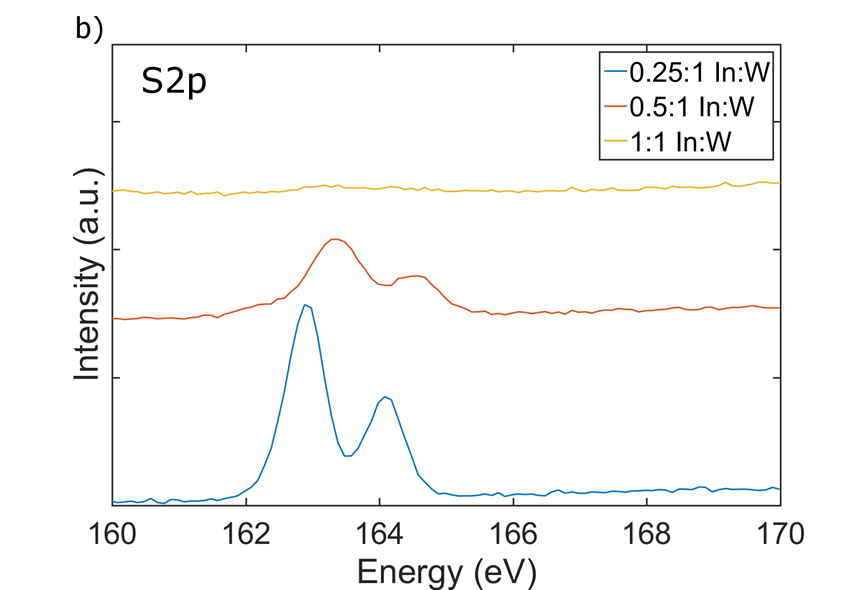
\includegraphics[width=\textwidth]{In/XPSS2p.png}
			\caption{S 2p}
			\label{fig:InXPSS2p}
		\end{subfigure}
		\begin{subfigure}[b]{0.6\textwidth}
			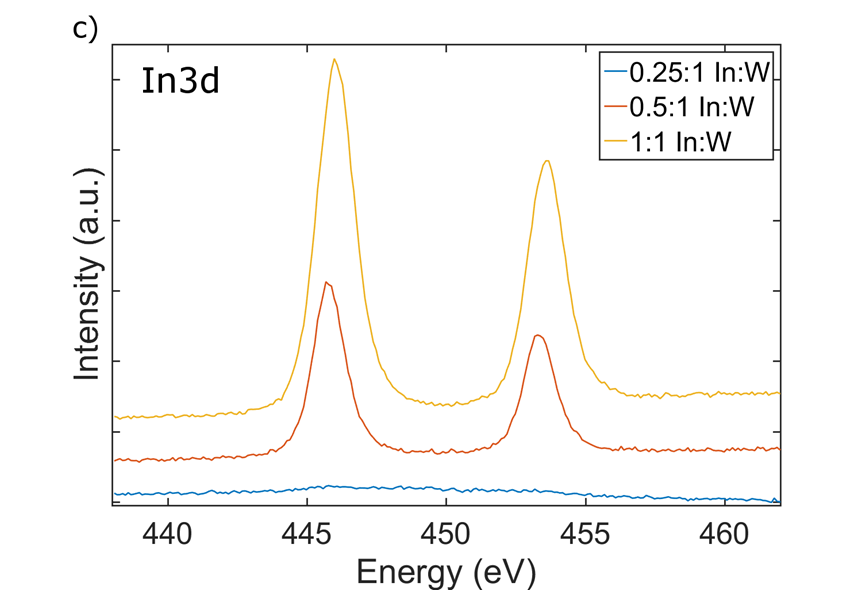
\includegraphics[width=\textwidth]{In/XPSIn3d.png}
			\caption{In 3d}
			\label{fig:InXPSIn3d}
		\end{subfigure}
		\caption{XPS spectra comparison}
		\label{fig:InXPSSpectra}
	\end{center}
\end{figure}

Figure \ref{fig:InXPSSpectra} shows the In 3d, W 4f and S 2p core levels XPS spectra for pure $WS_2$ and In-doped $WS_2$ (In/W=0.25, In/W=0.5, In/W=1). It can be noticed that, while pure $WS_2$ and $In_{0.25}WS_2$ do not exhibit any Indium core level peak (Figure \ref{fig:InXPSIn3d}), the samples In/W=0.5 and In/W=1 show In 3d5/2 and In 3d3/2 core levels at binding energies of ~444.8 eV and ~452.4 eV, respectively. Further, it is observed that both W4f core levels for the sample In/W=1 are slightly shifted to higher binding energies compared to the sample In/W=0.5 (Figure \ref{fig:InXPSW4f}), which can be attributed to the presence of $In_xW_yS_z$ compounds \cite{Wagner1991}. The peak shoulders at $\sim$443 eV and $\sim$451 eV observed for both samples In/W=1(2) and In/W=1(3) (Figure \ref{fig:InXPSW4f}) are due to the presence of $In_2S_3$. The W 4f5/2 and W 4f7/2 core levels peaks (Figure \ref{fig:InXPSW4f}) of the 1:1 In-doped samples are significantly shifted to higher energies compared to pure $WS_2$. 3 samples show similar shift of about 1.5 eV which may suggest the presence of $W^{6+}$ in the doped samples as opposed to $W^{4+}$ in pure WS2. This suggest a preferential bonding between In and W. One of the 1:1 samples exhibits even greater shift of about 4 eV which indicates presence of $WO_3$. 

Further, the S 2p1/2 and S 2p3/2 core levels peaks (Figure \ref{fig:InXPSS2p}) of the In/W=1 samples also appear at lower energies than pure $WS_2$ (S 2p1/2 and S 2p3/2 at 162 eV and 163.5 eV respectively). Thus, we can conclude that In atoms have been successfully interacting with $WS_2$ as there is a clear In-W interaction based on the In 3d and W 4f peak shifts. The In atoms are thus likely to be chemisorbed onto the $WS_2$ or incorporated into the layer as an interstitial. Table \ref{tab:InRatios} reports the stoichiometric ratios of In, W and S for the doped samples obtained by calculating the corresponding concentrations from the integrated intensity of the In 3d, W 4f and S 2p core levels. 

\begin{table}[!ht]
\caption{In:W and S:W ratios obtained by calculating the In, W and S concentrations from the integrated intensity of the In3d, W4f and S2p core levels.}
\label{tab:InRatios}
\end{table}

\begin{center}
\begin{tabular}{c|cc}

Sample 		& In/W 		& S/W\\\hline
In/W = 0.25 & 0.038:1 	& 2.32:1\\
In/W = 0.5	& 0.45:1	& 2.22:1\\
In/W = 1	& 1.98:1	& 0.27:1

\end{tabular}
\end{center}

The XRD diffraction patterns of all the In-doped $WS_2$ samples can all be indexed on a hexagonal unit cell basis (Figure \ref{fig:InXRDAll}) and they display a marked analogy to that of $2H-WS_2$. The most intense reflection is the (002) and for pure and In-doped $WS_2$ (Figure \ref{fig:InXRDIn}) it can be seen that the FWHM decreases as the In precursor concentration increases and that a peak shift towards a larger d spacing (Table \ref{tab:InXRDData}) occurs for the highest indium content. Further, the indium content of In/W=0.5, In/W=0.75 and In/W=1 show an additional reflection at $2{\Theta}=13.44$ not belonging to $WS_2$, which we attribute to the incorporation of In atoms into the $WS_2$ lattice.

\begin{table}[!ht]
\caption{Data for the (002) XRD peak and lattice parameters for pure $WS_2$ and In-doped $WS_2$ samples.}
\label{tab:InXRDData}
\end{table}

\begin{center}
\begin{tabular}{c|ccccc}

Sample 		& Position (2$\Theta$)	& FWHM (2$\Theta$)	& a (\r{A})	& c (\r{A})	& d (\r{A})	\\\hline
$WS_2$	 	& 14.44 				& 0.703				& 3.23		& 11.02		& 5.51		\\
In/W = 0.25	& 14.47					& 0.294				& 3.23		& 11		& 5.50		\\
In/W = 0.5	& 14.444				& 0.168				& 3.22		& 11.02		& 5.51		\\
In/W = 0.75	& 14.479				& 0.137				& 3.22		& 11		& 5.50		\\
In/W = 1	& 14.307				& 0.182				& 3.21		& 11.14		& 5.57

\end{tabular}
\end{center}

Therefore, it can be concluded that the crystal structure remains unchanged for Indium content of less than 0.038, corresponding to a precursor ratio of In/W = 0.25. For large indium contents an expansion of the van der Waals gap is observed due to the large amount of indium intercalated between the layers in few-layered regions and also a small portion of indium can result incorporated in the crystal structure. 

Our results are in agreement with earlier studies on the In intercalation in bulk $MoS_2$ which revealed that large metal ions, such as In and Ga, are likely to retain the hexagonal structure of $MoS_2$ on the contrarily of small ions in the form of alkali and alkaline earth metals, which mostly lead to a modification of the crystallographic order \cite{Somoano1979} to the octahedral coordination. The presence of d-bands in indium metal provide an additional contribution to bonding stabilization.
 

\begin{figure}[!h]
	\begin{center}
		\begin{subfigure}[b]{0.7\textwidth}
			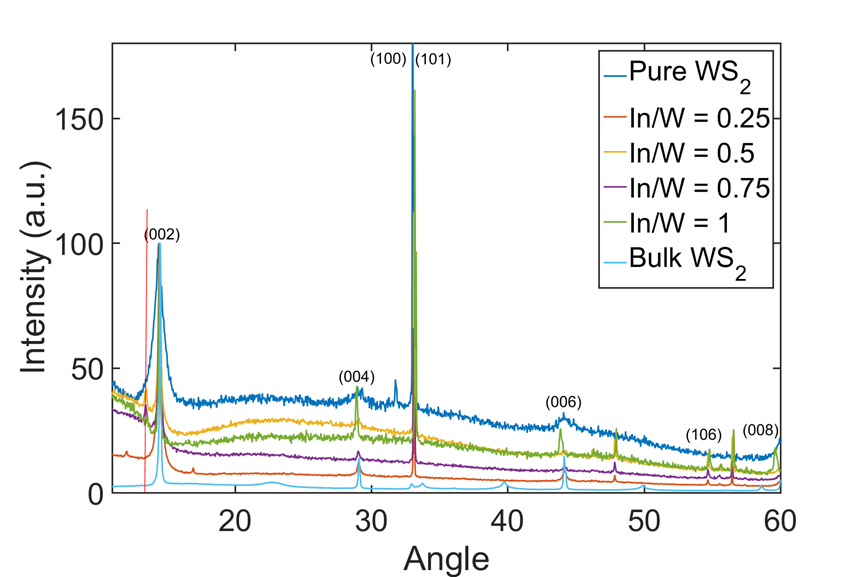
\includegraphics[width=\textwidth]{In/XRDAll.png}
			\caption{XRD patterns for CVD-grown pure $WS_2$ and In-doped $WS_2$.}
			\label{fig:InXRDAll}
		\end{subfigure}
		\qquad
		\begin{subfigure}[b]{0.7\textwidth}
			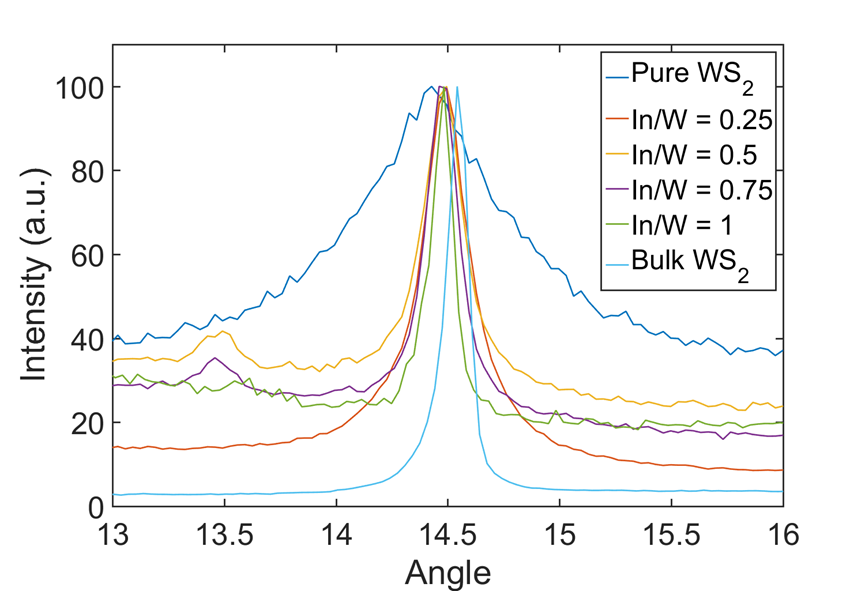
\includegraphics[width=\textwidth]{In/XRDIn.png}
			\caption{(002) XRD peak for CVD-grown pure $WS_2$ and In-doped $WS_2$}
			\label{fig:InXRDIn}
		\end{subfigure}
		\caption{XRD spectra of $WS_2$ samples}
		\label{fig:InXRDSpectra}
	\end{center}
\end{figure}

\begin{figure}[H]
	\begin{center}
		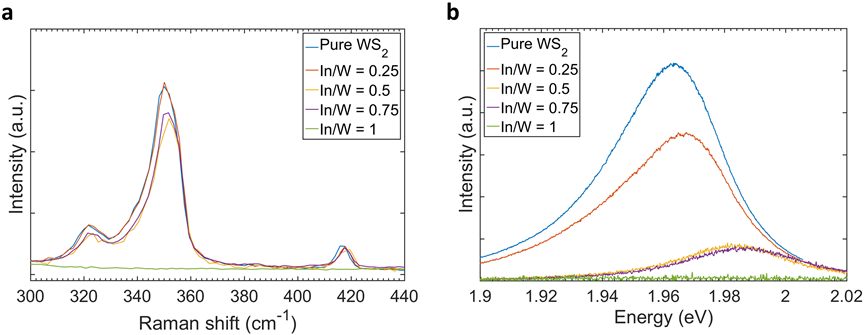
\includegraphics[scale=0.5]{In/RamanPL.png}
		\caption{Representative a) Raman and b) PL spectra for pure $WS_2$ (grown by using $H_2WO_4$ as metal precursor) and In-doped $WS_2$}
		\label{fig:InRamanPL}
	\end{center}
\end{figure}

Additionally, the reflections at $2\Theta ={\sim}48$ and $\sim$57 have been ascribed to the presence of $In_2S_3$ \cite{Hahn1949} and specifically for the planes (002). This has been observed in the form of thick crystals in the centre of atomically thin flakes (Figure \ref{fig:InSEMCentre}) and as ascertained by Raman spectroscopy (Figure \ref{fig:InSEMCentre}). Since $In_2S_3$ flakes are rarely found and they present a low nucleation density compared to the $WS_2$ domains, thus they can be considered as secondary reaction products.

\begin{figure}[!h]
	\begin{center}
		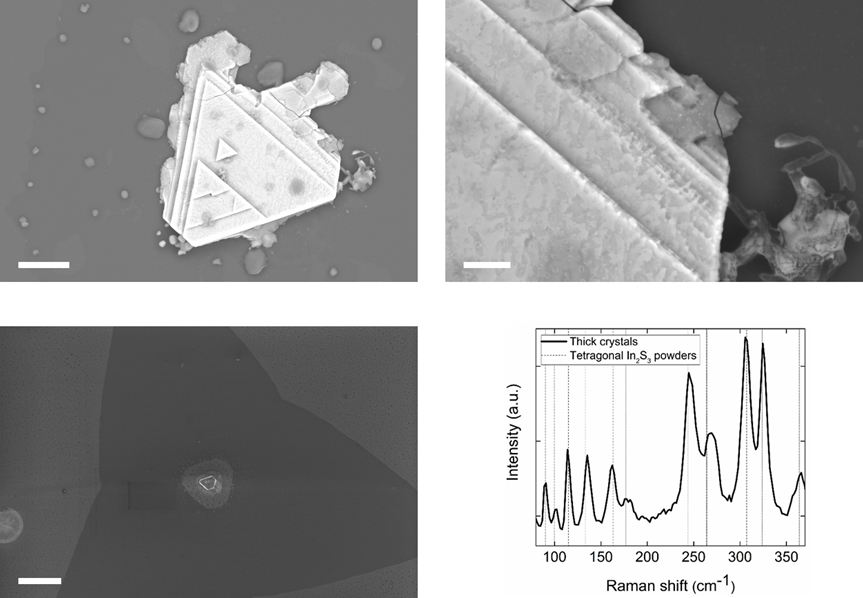
\includegraphics[scale=0.5]{In/SEMCentre.png}
		\caption{Low-magnification SEM images in (a) SE and (b) BSD imaging mode of the same area of sample In/W=1. High-magnification SEM images in (c) SE and (d) BSD imaging mode of the same area of sample In/W=1, revealing compositional variation across the flakes}
		\label{fig:InSEMCentre}
	\end{center}
\end{figure}

The representative Raman spectra for undoped WS2 and In-doped WS2 are reported in Figure \ref{fig:InRamanPL} a). It can be observed that $WS_2$ with In content between 0.038-0.45 show the characteristic in-plane 2LA-$E^1_{2g}$ and out-of-plane $A_{1g}$ vibrational Raman active modes of $WS_2$, while Indium content of 1 is not Raman active. Similarly, $WS_2$ with In content between 0.038-0.45 exhibit PL while $WS_2$ with In content of 1 does not luminescence (Figure \ref{fig:InRamanPL} b)). Therefore, a very large amount of In (equal to 1) alters the crystal structure and properties of the host material. This has been also confirmed by XPS and electrical measurements. The $E^1_{2g}$ and $A_{1g}$ Raman peaks (Figure 2c) of all of the In-doped samples (In/W=0.25, In/W=0.5 and In/W=0.75) are shifted towards higher frequencies ($E^1_{2g}$ at $~351.5cm^{-1}$ and $A_{1g}$ at $~418^{cm-1}$) as compared to pure $WS_2$. This could be due to the differences in the binding energy between W–S and (W-In)–S bonds. Nevertheless, the shifts in Raman frequencies observed in atomically thin metal-doped TMDCs is not yet fully understood and further studies are needed. The excitons-to-trions ratio (Figure \ref{fig:InPLRatioHistogram}) for all the PL active In-doped samples (In/W=0.25, In/W=0.5 and In/W=0.75) is lower than that of pure $WS_2$, thus indicating an increase of the n-type doping with the In concentration. This trend may be explained considering that the post-transition In metal atoms have fully-filled d-orbitals and an additional third electron in a p-orbital in the most outer shell. This excess electron may thus enhance the concentration of electrons in the n-doped $WS_2$, which leads to a semiconducting-to-metallic transition of the host material at high In incorporation levels. This trend has been confirmed by electrical characterization of the $InWS_2$, which showed an increase in the resistance with increasing temperature, thus revealing a metallic-type behaviour (Figure \ref{fig:InElectricalMeasurement}).

\begin{figure}[!h]
	\begin{center}
		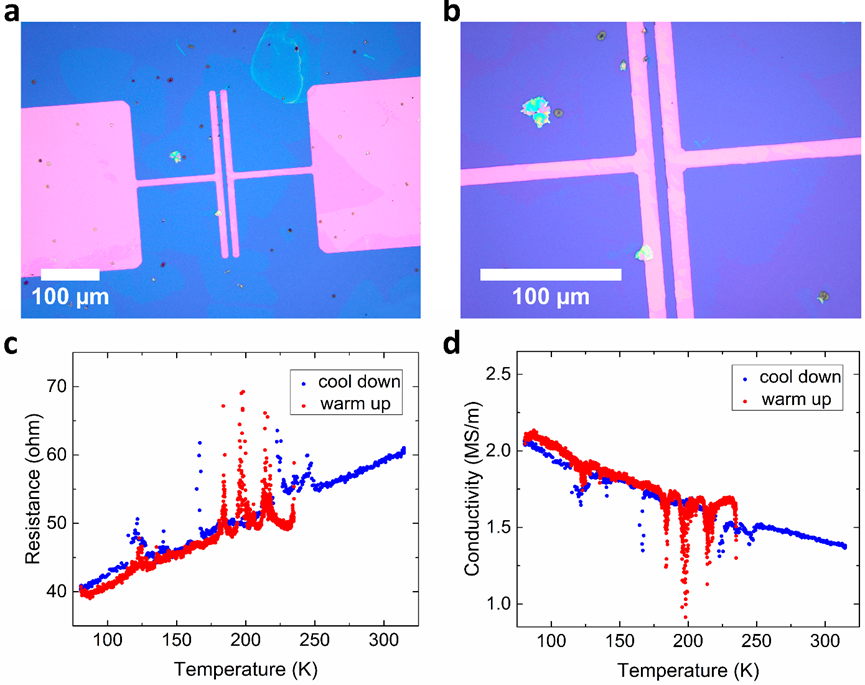
\includegraphics[scale=0.5]{In/ElectricalMeasurements.png}
		\caption{(a, b) Optical micrographs of Ti and Au contacts deposited on In/W=1 flakes. (c) Measured resistance as a function of temperature. (d) Calculated conductivity vs. temperature revealing a semi-metallic behaviour.}
		\label{fig:InElectricalMeasurement}
	\end{center}
\end{figure}

\newpage
\begin{figure}[!h]
	\begin{center}
		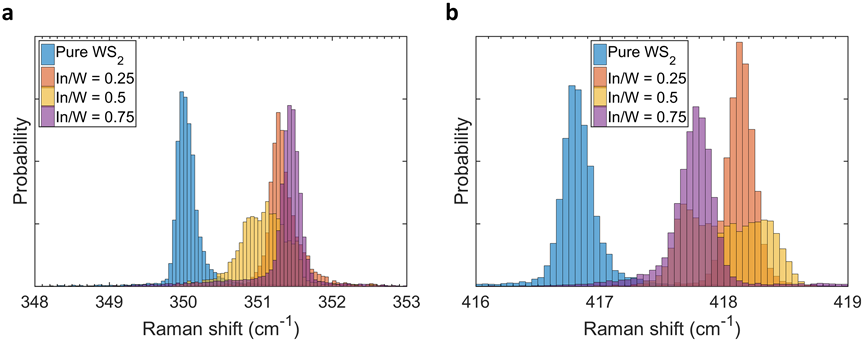
\includegraphics[scale=0.5]{In/RamanPositionHistogram.png}
		\caption{a) $E^1_{2g}$ and b) $A_{1g}$ peak positions for pure $WS_2$ and Raman active In-doped $WS_2$ samples.}
		\label{fig:InRamanPLHistogram}
	\end{center}
\end{figure}

\begin{figure}[H]
	\begin{center}
		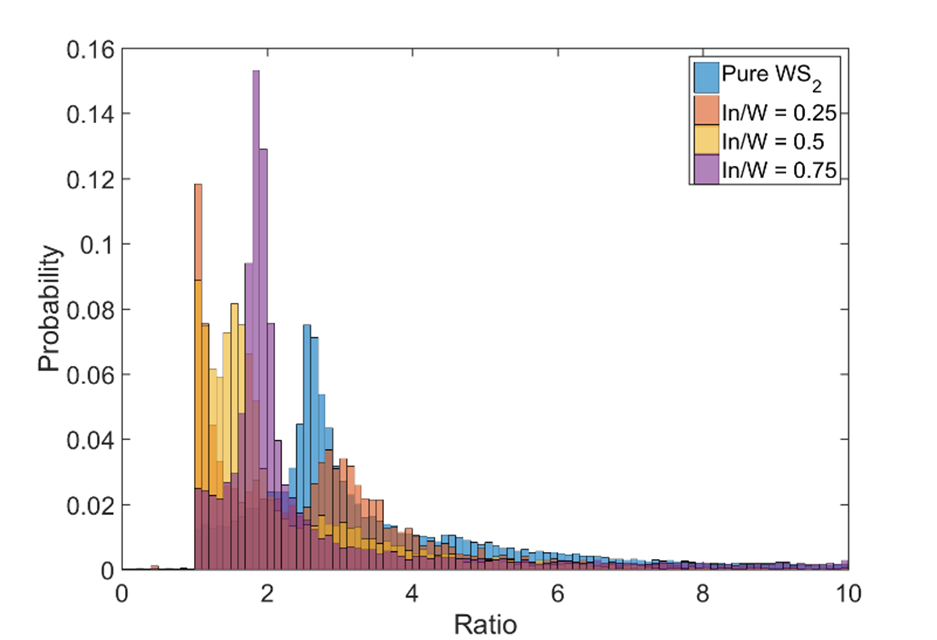
\includegraphics[scale=0.4]{In/PLRatioHistogram.png}
		\caption{Excitons-to-trions ratio for pure $WS_2$ and PL active In-doped $WS_2$ samples XPS}
		\label{fig:InPLRatioHistogram}
	\end{center}
\end{figure}

%%%%%%%

The sample with In:W growth ratio of 0.5:1 was further analysed using transmission electron microscopy (TEM). In order to prepare the samples for the measurement the as grown flakes of $WS_2$ on $SiO_2/Si$ have to be transferred onto a TEM grid made of thin (200 nm) carbon layer stretched across copper grid. The samples were therefore transferred using the standard wet transfer method described in chapter \ref{cha:Transfer}. Due to irregular surface of TEM grid consisting of shallow holes as well as delicate carbon film the wet transfer method proved to be less efficient than when transferring onto a flat $SiO_2/Si$ surface. Due to acetone bath and several steps of heating and cooling the carbon film breaks in many places leading to partial loss of the transferred material. The TEM images of the transferred $WS_2$ flakes can be seen in Figure \ref{fig:InTEMImages}. The contrast in those images is primarily caused by the size of the atoms with smaller atoms of C contributing very little and being barely distinguishable from an empty space, while the bigger W atoms resulting in much more noticeable contrast. The Figure \ref{fig:InTEMImage1} shows relatively thick $WS_2$ flake of $<10$ layers with some smaller areas of more layers. The Figure \ref{fig:InTEMImage2} shows a folded and crumpled flake with thickness ranging from few, 2-3 layers up to very thick. There is also a thin, flat flake on the right side which retained most of the triangular shape. In Figure \ref{fig:InTEMImage3} there is a larger crumpled flake seen across the image. In the center there is one corner of a thin, flat triangular flake.

\begin{figure}[H]
	\begin{center}
		\begin{subfigure}[b]{0.6\textwidth}
			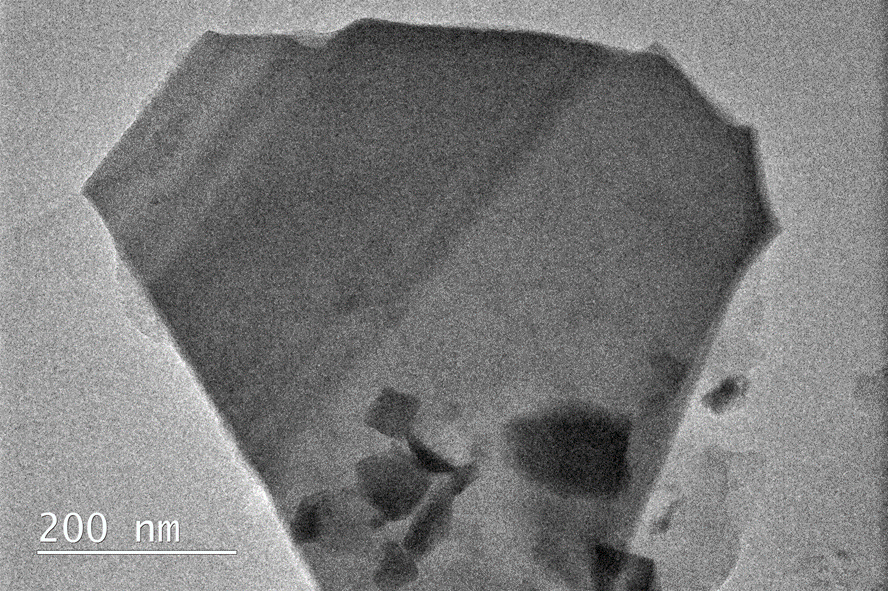
\includegraphics[width=\textwidth]{In/TEMImage1.png}
			\caption{}
			\label{fig:InTEMImage1}
		\end{subfigure}

		\begin{subfigure}[b]{0.6\textwidth}
			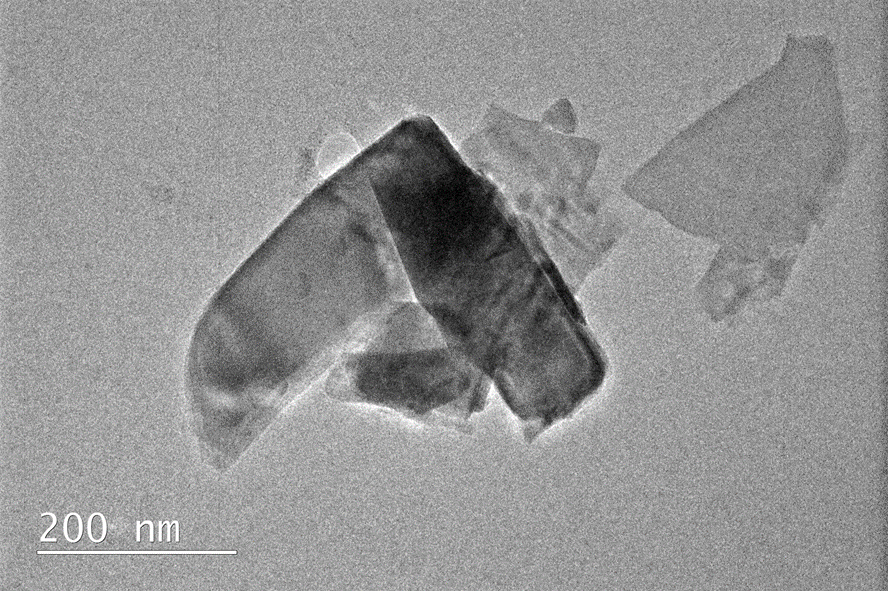
\includegraphics[width=\textwidth]{In/TEMImage2.png}
			\caption{}
			\label{fig:InTEMImage2}
		\end{subfigure}

		\begin{subfigure}[b]{0.6\textwidth}
			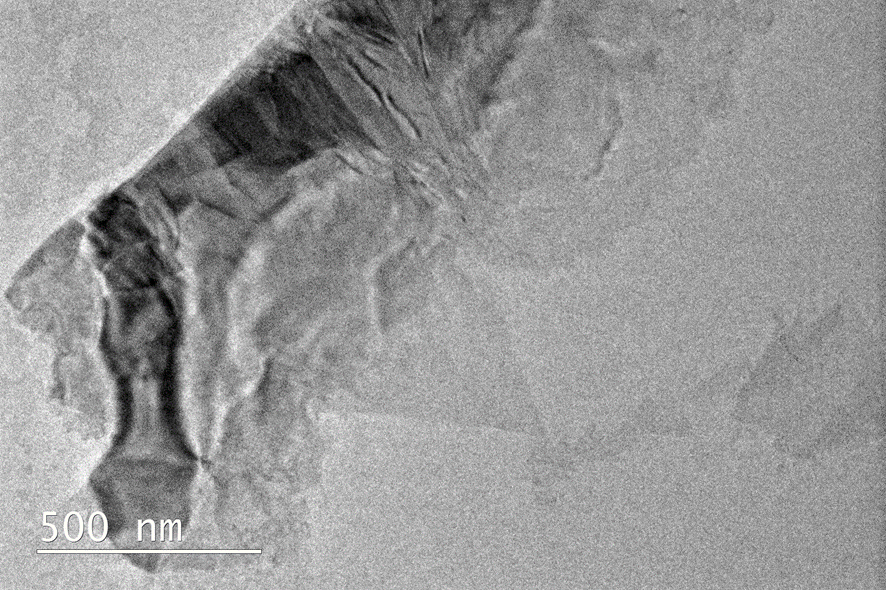
\includegraphics[width=\textwidth]{In/TEMImage3.png}
			\caption{}
			\label{fig:InTEMImage3}
		\end{subfigure}
		\caption{TEM images of the $WS_2$ sample with $In:W = 0.5:1$}
		\label{fig:InTEMImages}
	\end{center}
\end{figure}

The energy dispersive x-ray spectroscopy (EDS) has been then utilised to find the chemical makeup of the sample. First the as grown sample was characterised using SEM EDS which requires no sample transfer. As seen in Figure \ref{fig:InTEMEDSFra} there are In peaks present at: $L_{{\alpha}1} = 3286.94; L_{{\alpha}2} = 3279.29; L_{{\beta}1} = 3487.21; L_{{\beta}2} = 3713.81; L_{{\gamma}1} = 3920.81$. This indicates that there is some In in, on or around the $WS_2$ flake. There is also visible $Na$ peak which indicates remaining $Na$ from $NaCl$ used for synthesis. In order to compare the as grown sample, the transferred sample was characterised using TEM EDS. AS seen in Figure \ref{fig:InTEMEDS} there is no visible In peak. This indicates that the In is somehow removed during the transfer process. It is therefore most likely that the In is not present inside the $WS_2$ as a dopant, as substitution or an interstitial, or that it is located in between the layers, but that it is present on top of or around the as grown $WS_2$ flake.

\begin{figure}[H]
	\begin{center}
			\begin{subfigure}[b]{0.6\textwidth}
			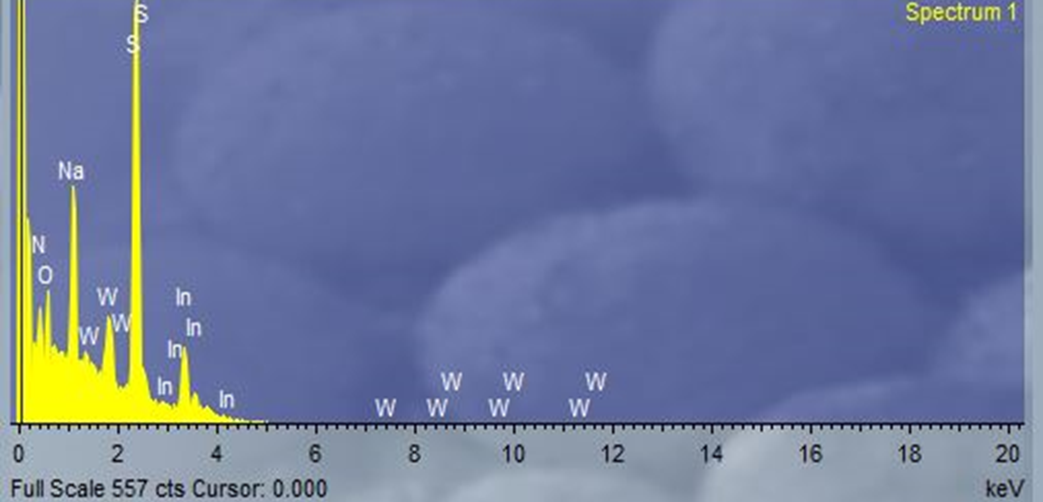
\includegraphics[width=\textwidth]{In/TEMEDSFra.png}
			\caption{Before transfer}
			\label{fig:InTEMEDSFra}
		\end{subfigure}
		\qquad
		\begin{subfigure}[b]{0.6\textwidth}
			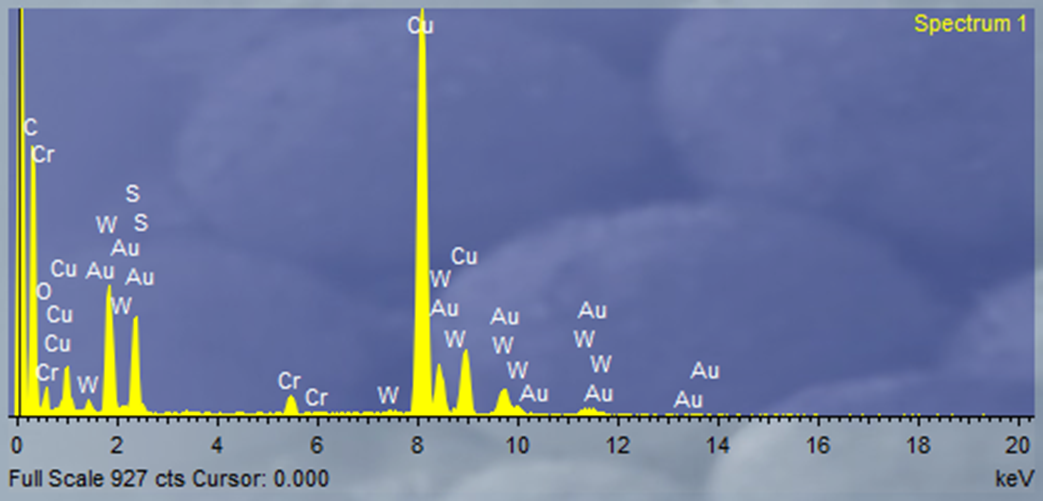
\includegraphics[width=\textwidth]{In/TEMEDS.png}
			\caption{After transfer}
			\label{fig:InTEMEDS}
		\end{subfigure}
		\caption{EDS spectra collected using TEM from $WS_2$ sample with $In:W = 1:2$}
		\label{fig:InTEMEDSSpectra}
	\end{center}
\end{figure}

Additionally the electron diffraction (ED) measurement was performed. As seen in Figure \ref{fig:InTEMED} the present pattern correspond to the expected pattern for $WS_2$. The spots are sharp and narrow indicating mostly monolayer $WS_2$ with no elongation or broadening expected due to the presence of irregular presence of doping element. There is also no additional pattern that could indicate a super structure of ordered atoms of the dopant. The faint halo indicates presence of the amorphous carbon of the TEM grid. The faint signal is therefore indicative of a lack of polymer remains after the transfer. Finally the calculated lattice parameter $a$ was found to be a = 2.71 \r{A} which is in agreement to the $a$ parameter found for the un doped $WS_2$ from the XRD spectrum as seen in Figure \ref{fig:InXRDSpectra} (a = 2.71 \r{A}) as well as the  one found for the bulk $WS_2$ (a = 2.73 \r{A}). This indicates therefore that the transferred sample shows no change in strain after the transfer.

\begin{figure}[H]
	\begin{center}
		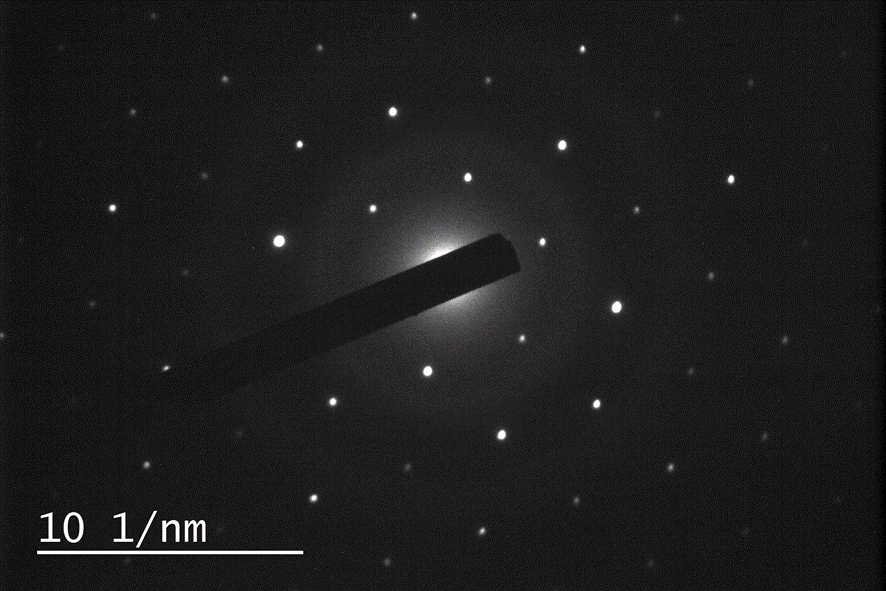
\includegraphics[scale=0.4]{In/TEMED.png}
		\caption{Electron diffraction pattern of $WS_2$ flake with $In:W = 1:2$}
		\label{fig:InTEMED}
	\end{center}
\end{figure}

\section{Conclusions}

In summary, we have reported indium atoms doping of $WS_2$ atomic layers in situ during synthesis, without sacrificing the lateral extension or the reproducibility of the synthesis process. Remarkably, the In-doped $WS_2$ samples exhibit tunable light emission and a semiconducting-to-semimetallic transition at high doping levels. Therefore, the present synthesis strategy can be employed to achieve tailorable optical and electrical characteristics of atomically-thin $WS_2$ through stable incorporation of non-volatile post-transition metal atoms.